\chapter{System design plan} \label{chap:system_design}
In this chapter I'm introducing the planned steps towards building the previously described system. Due to the 
COVID-19 outbreak I have no access to the university laboratory when writing this thesis and therefore the planned 
system cannot be built physically. 

TODO

\section{VL53L1X measurements} \label{sect:vl53l1x_measurements}
In order to simulate the chosen VL53L1X sensor accurately, experience needs to be gained using the device. 
There are several factors that affect the quality of the map produced by the SLAM algorithm. Choosing the right
settings for the LIDAR sensor therefore is a crucial part that cannot be determined independently from the SLAM 
algorithm. At this point it is unsure if what resolution, low maximum distance but higher sampling rate is beneficial 
for SLAM algorithm or the other way around. My approach is to first explore the capabilities of the sensor in 
all relevant operating modes, measure the ranging performance like update rate, maximum ranging distance and 
noise level of the measurements. Later on the optimal operating mode can be chosen based on the SLAM performance. 

\begin{figure}[!hb]
    \centering
    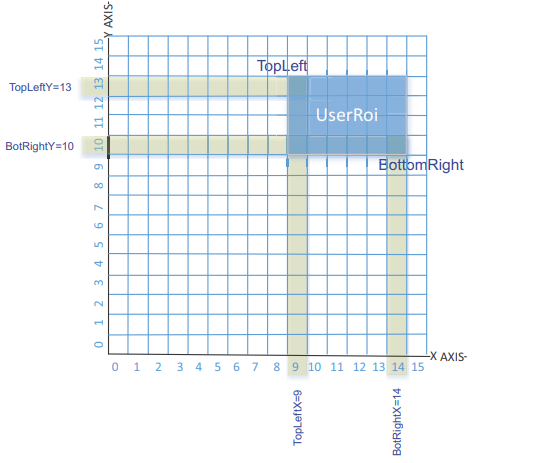
\includegraphics[width=90mm, keepaspectratio]{figures/vl53l1x_roi_setup.png}
    \caption{VL53L1X Region of Interest setting \cite{VL53L1XApplicationNote}}
    \label{fig:vl53l1x_roi_setup}
\end{figure}

The sensor has three parameters, that affect the ranging performance and require tuning for each application. 
These three parameters are the distance preset, the timing budget and the Region of Interest(ROI). The device 
has three different distance presets for short, medium and long distance ranging. The second parameter is the
timing budget, that basically sets how much time is available for the sensor to complete a range. Bigger 
timing budget means more accurate measurement, but on the downside it lowers the sampling rate.

As described in section \ref{sect:vl53l1x_intro} the sensor has a configurable SPAD array that can be used to 
narrow down the field of view to a specific region. This region in the datasheet is called Region of Interest
and will be further referenced to as ROI. By lowering the size of the ROI and changing its position, scanning 
can be achieved resulting in a higher resolution up to 4x4. Increased resolution means smaller receiving array 
that lowers sensitivity and maximum distance that can be measured. Scanning also requires more time because 
each ROI can take time up to the timing budget.

\begin{figure}[!ht]
    \centering
    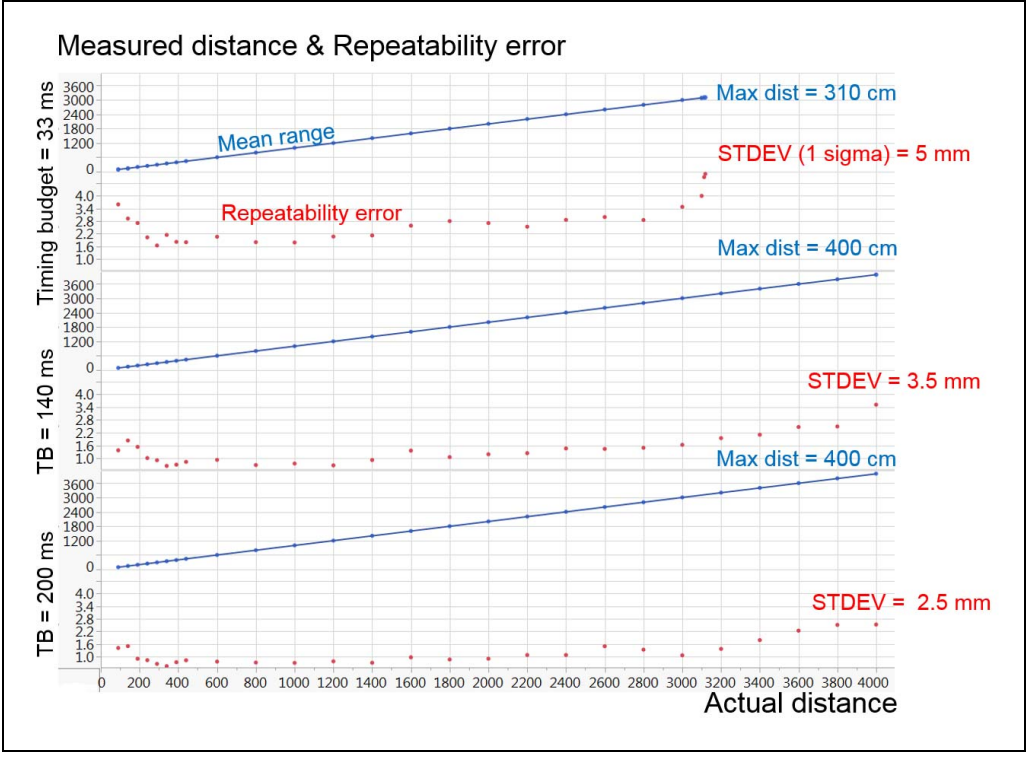
\includegraphics[width=140mm, keepaspectratio]{figures/vl53l1x_timing_budget.png}
    \caption{VL53L1X maximum distance, error vs timing budget \cite{VL53L1XDatasheet}}
    \label{fig:vl53l1x_timing_budget}
\end{figure}

\subsection{Selected operating modes}
To have a better overview how these parameters affect the ranging performance, a number of operating modes 
have been chosen for testing. Each operating mode is a group of three parameters that are the distance preset,
timing budget and the resolution. The performance of an operating mode is measured by the update rate, maximum 
ranging distance and standard deviation on a given distance.

According to the VL53L1X datasheet, the 4m maximum distance can only be achieved in long preset, 3m in medium 
and 1.3m in short. The datasheet contains a plot for maximum distance, standard deviation vs timing budget
in long ranging preset with ROI set to maximum size. The timing budgets in the datasheet are 33ms, 
140ms and 200ms, therefore I have selected these timings for test measurements. 

As an additional setup an operating mode with the highest update rate has been selected, because update rate is
expected to improve SLAM performance. This can be achieved by using an inter-measurement period of 20ms and 
timing budget of 18.5ms, but only in short range preset and ROI size set to maximum. The estimated highest 
update rate using this operating mode is 50Hz.

\begin{figure}[!ht]
    \centering
    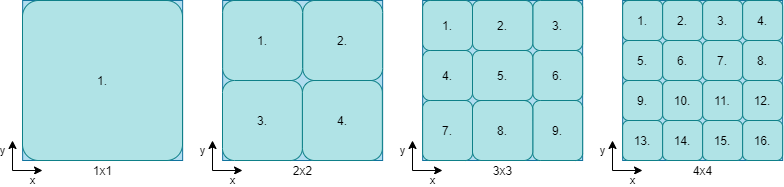
\includegraphics[width=150mm, keepaspectratio]{figures/vl53l1x_spad_arrays.png}
    \caption{VL53L1X ROI setups}
    \label{fig:vl53l1x_spad_arrays}
\end{figure}

As seen on figure \ref{fig:vl53l1x_timing_budget} that the sensor provides measurements with a standard deviation
under 5mm, but it's not mentioned how the accuracy changes by lowering the ROI size. To investigate the 
performance of ranging measurements using lower ROI size, four Region of Interest scan patterns have been selected.
The regions are selected evenly on the SPAD array to provide 1x1, 2x2, 3x3, 4x4 resolution output. These setups 
have been selected, because this way the regions do not overlap and are evenly distributed. The sensor would be
capable of more complex patterns or even changing the resolution between scans, but these setups should provide 
a good understanding of the sensor and the effects on the SLAM performance.

\begin{table}[ht]
	% \footnotesize
	\centering
	\begin{tabular}{||c c c c||}
		\hline
        Timing budget       & Resolution        & Range preset      & Distance  \\
		\hline\hline
        18.5 ms      & 1x1, 2x2, 3x3, 4x4      & Short      & 1 m \\
		\hline
        33 ms        & 1x1, 2x2, 3x3, 4x4      & Medium, Long       & 1 m \\
		\hline
        140 ms       & 1x1, 2x2, 3x3, 4x4      & Medium, Long       & 2.5 m \\
		\hline
        140 ms       & 1x1, 2x2, 3x3, 4x4      & Medium, Long       & 3 m \\
		\hline
        140 ms       & 1x1, 2x2, 3x3, 4x4      & Long       & 3.5 m \\
		\hline
        200 ms       & 1x1, 2x2, 3x3, 4x4      & Long       & 3.5 m \\
		\hline
	\end{tabular}
	\caption{Selected operating modes}
	\label{tab:selected_operating_modes}
\end{table}

In table \ref{tab:selected_operating_modes} a summary can be found of selected operating modes and a 
distance to be tested on. These settings are planned to be evaluated incrementally starting with a 
timing budget of 18.5ms and incrementally moving up to 200ms. With smaller ROI size the maximum 
distance is degrading, therefore it is expected that some combinations will not be working 
properly. For example medium preset on 3 meters is expected to be working only on resolution 1x1, 
but likely to fail on higher resolutions.








\section{LIDAR layout} \label{sect:lidar_layout_plan}
As mentioned before, multiple aspects need to be taken into account when placing LIDAR sensors on a
quadcopter with the purpose of using the measurements for SLAM. After gaining experience of the performance
of each operation mode of the sensor, the next step is to determine the optimal layout and number of sensors 
to be used. 

In Cartographer 3D SLAM is basically an extension of their 2D solution, but significantly more complex and 
harder to tune for optimal performance. With this in mind to better understand the effects of
layout it is reasonable to first reduce complexity and test layouts for 2D mapping. Based on 
the experience gained during this experiment it can be better estimated how many sensors and in what layout
are needed for 3D SLAM. A possible outcome is that VL53L1X is not suitable at all for this purpose and
a different sensor needs to be used, with more suitable parameters. If mapping and localization accuracy 
is poor in 2D, it is expected to be worse in 3D.

\subsection{Layout design for 2D SLAM}
Without experience with Cartographer or other SLAM algorithms in general, it is not advisable to give an 
estimation for the number of sensors to be used or the layout of the sensors at this point. My approach 
is to start with high number of sensors in a reasonable layout, make it work with Cartographer and then
incrementally decrease the number of sensors until the result is still acceptable.

For 2D SLAM I chose to place LIDARs evenly to cover the whole 360$^{\circ}$ range of the horizontal plane, 
without overlapping fields of the sensors. Due to the high sampling rate and parallel ranging operations, 
overlapping fields could would have a higher probability of crosstalk between neighbors and would produce 
additional noise in real-world applications, that is better to avoid. Altogether 13 sensors are needed to 
cover 97.5\% of the plane, with 27.69$^{\circ}$ in between, leaving lass 1$^{\circ}$ of uncovered zone in 
between fields. 13 sensors can produce 13 points per scan with ROI resolution set to 1x1 and up to 208 
points with the resolution set to 4x4. 

\begin{figure}[ht]
    \centering
    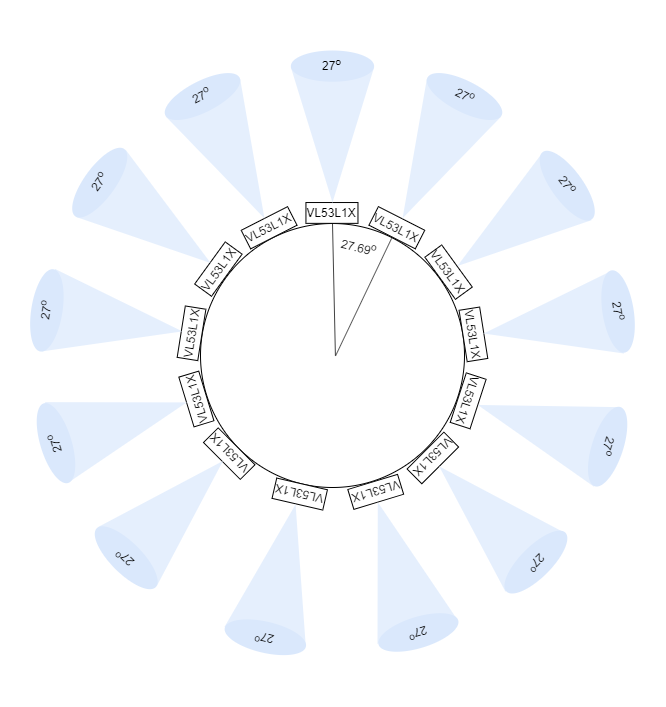
\includegraphics[width=70mm, keepaspectratio]{figures/2d_slam_13sensors.png}
    \caption{Layout of 13 LIDAR sensors}
    \label{fig:2d_13sensor_layout}
\end{figure}

In this layout the scanning on the horizontal plane is done purely by the evenly placed the sensors 
around the vertical axis and doesn't take advantage of the movement of the drone during flights, especially 
turns around the yaw axis. After evaluating the performance of this layout, the number of sensors will be
incrementally decreased, by removing a number of sensors at a time. The reduced set of sensors will always
be placed evenly, because multicopters can fly in any direction. The flying style is highly dependent on the
pilot, so it is best to scan the plane evenly without assuming any dominant flying direction.

The planned bottom limit for the number of sensors is what can be seen on the solution of Bitcraze, 
the Multi-ranger deck\cite{BitcrazeMultirangerDeck} that uses 4 sensors on the horizontal plane facing forward, 
backwards, left and right. In their demonstration video, the map of a simple room is built in 20 seconds 
with a ranging frequency of about 10Hz. 

\subsection{Layout design for 3D SLAM}
The layout for 3D SLAM depends on the experience gained during the evaluation of 2D SLAM, but has more 
freedom in sensor placement. Because multicopters change their pitch and roll angles to move horizontally,
this movement can be used for scanning of the vehicle's environment. 

Just like in case of 2D SLAM, in the first layout sensors are placed evenly to cover the whole sphere,
without overlapping fields. In the following iterations a number of sensors will be removed until the 
minimum number of sensors is found that still provide a reliable SLAM performance.



\section{Data collection in Gazebo Simulator}
To compare the performance SLAM setups using different layouts and operating modes, I have decided to 
work on the same set of data in each iteration. ROS offers a great tool to record data that is being 
transferred in ROS topics into a format that they call rosbag. This tool subscribes to the requested
topics and saves all ongoing data into a file with .bag extension. The same tool can be used to play 
back previously recorded data and the tool will publish messages at the same rate as it was 
published originally. ROS also provides a C++ and a Python application programming interface for rosbags
that can be used to read or write the contents of a bag file.

My plan is to place a high resolution 360$^{\circ}$ LIDAR sensor that covers the whole sphere
on a simulated quadcopter, fly it around in a building while recording the necessary topics into a rosbag.
The ranges in this rosbag can be then filtered in a way, that its parameters match the selected operation 
mode and layout. This way the performance of the SLAM using different layouts and sensor operating modes
can be compared.



\subsection{Development environment in Visual Studio Code}
After building the repository using the guide on PX4 website, I have learned that new models, launch files
and world files need to be placed in a subdirectory of the repository that is only generated at build. This
also means that if the project is rebuilt, the newly added files might be overwritten. To avoid overwriting
on builds, I have started working on these files in a different folder and copy it to their final destination
just before starting the simulation. 

Cartographer also uses the same mechanism, all files need to be copied to subfolders in its install 
location. For editing these files I use Visual Studio Code and to make copying easier, I have decided 
to add a build task in my editor, that copies PX4 files and cartographer files to the corresponding folder.
This makes the development much easier and less troublesome.

The project folder structure can be seen on figure \ref{fig:vscode_folder_structure}. Measurements folder 
will contain the output of each SLAM configuration and simulation folder is for ongoing development. Under
simulation, the bag folder contains recorded and filtered bag files. All cartographer specific files are in
subfolders of cartographer\_files folder. 
Catkin\_ws folder holds the Cartographer\_ros repository and its 
dependencies. Firmware is for storing PX4 repository and firmware\_file contains custom files to be copied
to the PX4 build directory. QGC stands for QGroundControl, that is not necessary for this simulation, but
can be useful in some cases. Lastly scripts folder is for scripts that are used for rosbag filtering, 
trajectory extraction or other purposes.


\begin{figure}[!ht]
    \centering
    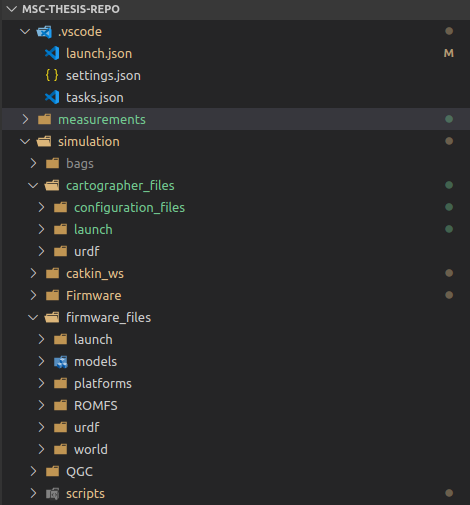
\includegraphics[width=70mm, keepaspectratio]{figures/vscode_folder_structure.png}
    \caption{Project folder structure in Visual Studio Code}
    \label{fig:vscode_folder_structure}
\end{figure}


\subsection{Adding LIDAR sensor to a quadcopter model}
Instead of overwriting files generated during the build procedure of PX4 repository, I have decided to 
create a custom quadcopter model, that extends the already available Iris drone. Any sensor that is 
supported Gazebo can be added to it, by editing the model descriptor SDF file. 

The equivalent of a LIDAR sensor in Gazebo is called a Ray sensor, that is highly customizable using
parameters in the SDF model file. The goal is that the rays of the sensor cover the whole sphere around 
the quadcopter. The rays of the LIDAR are blocked by the simulated drone so a single sensor
cannot be used to cover the whole sphere. 
I have placed two sensors on the drone, one on the top and one on the bottom as close to the body
of the vehicle as possible. 

Since the VL53L1X sensors in real-world application would be measuring simultaneously, the simulated 
LIDARs are also set to scan every angle at once and send all ranges in a single message. The maximum 
range is set to 4 meters and the update rate is at 50Hz. Gazebo is able to simulate predefined measurement
noise, but at first I have decided not to add additional noise. During data filtering these measured 
point clouds will be down-sampled by averaging on regions and noise can be simulated in addition at 
this stage. In each scan 128 horizontal and 64 vertical points are sampled per sensor, resulting in 
a total number of 128*128 measurement points and angular resolution of 2.8$^{\circ}$ both vertical 
and horizontal.

\begin{figure}[!ht]
    \centering
	$\vcenter{\hbox{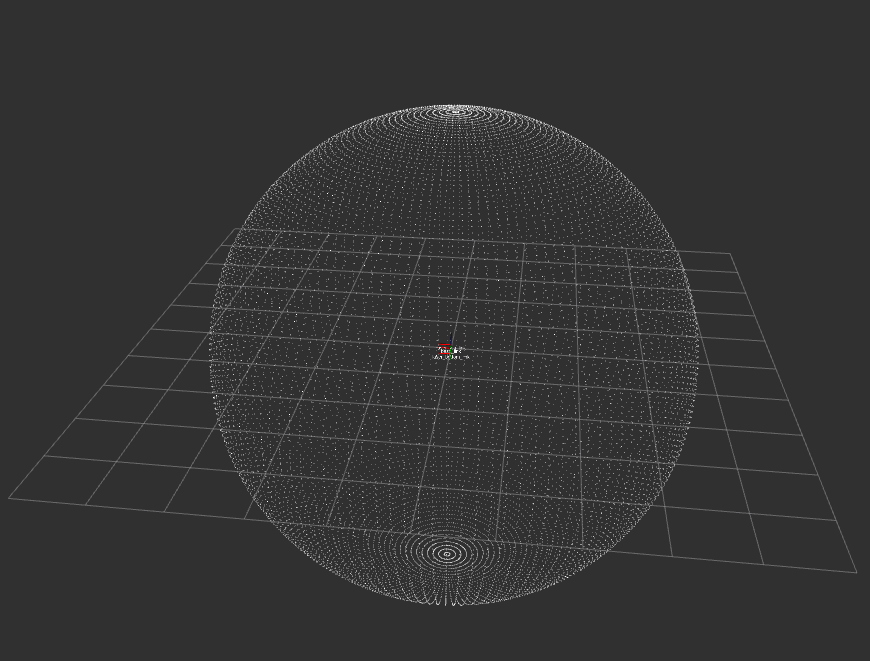
\includegraphics[height=57mm, keepaspectratio]{figures/lidar_simulation.png}}}$
    $\vcenter{\hbox{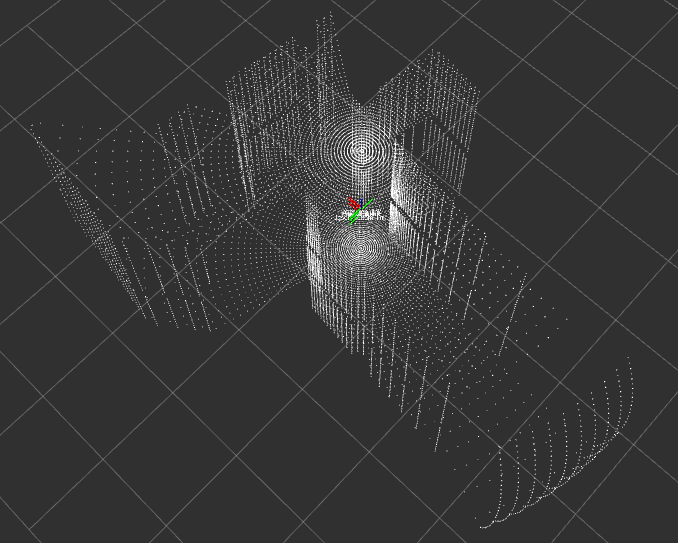
\includegraphics[height=57mm, keepaspectratio]{figures/lidar_simulation_2.png}}}$
    \caption{LIDAR output visualization in rviz}
    \label{fig:lidar_visualization_rviz}
\end{figure}

The maximum update rate of each simulated LIDAR is 30Hz, because Ray sensor uses the CPU for 
computations instead of the GPU. It would be possible to use an alternative called GPU Ray,
but I decided not to use it, because of its output message type. Cargorapher expects ranges aggregated
into PointCloud2 messages, while Ray sensor's output is PointCloud and the GPU alternative has an 
output in LaserScan format. PointCloud2 is a newer version of PointCloud and conversion is relatively
easy. If 30Hz update rate is proved to be too low during future steps, it is possible to use GPU 
Ray instead, that requires modifications in the filtering algorithm.


\subsection{Building model}
Using Gazebo Building Editor I have created a building model to be mapped. The building is minimalistic
and not furnished, but contains enough details like columns and curves to allow Cartographer to match 
scans more efficiently. For example SLAM is not expected not work properly on a corridor without any details
in range, because it needs a reference points that can be used for scan matching. If each scan looks exactly
the same the algorithm will lose track resulting in bad map quality. This is increasingly in focus in this
case, because the maximum distance of the VL53L1X sensor to be used is 4m and the sensor has a wide field 
of view that hides details of faraway objects.

\begin{figure}[!ht]
    \centering
	$\vcenter{\hbox{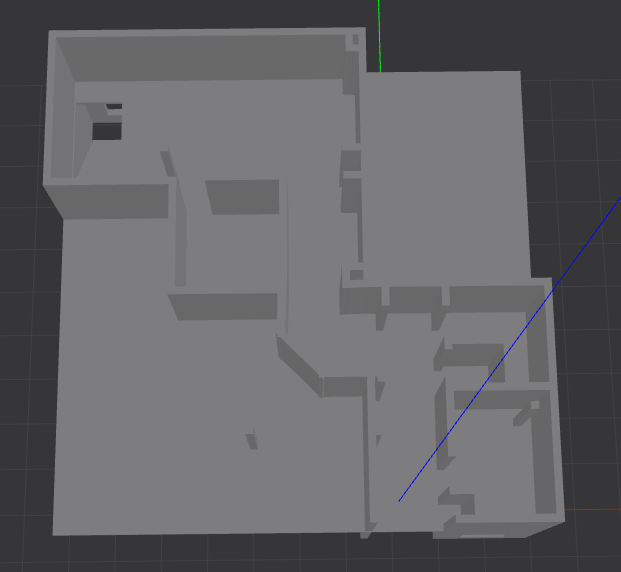
\includegraphics[height=62mm, keepaspectratio]{figures/building_1.png}}}$
    $\vcenter{\hbox{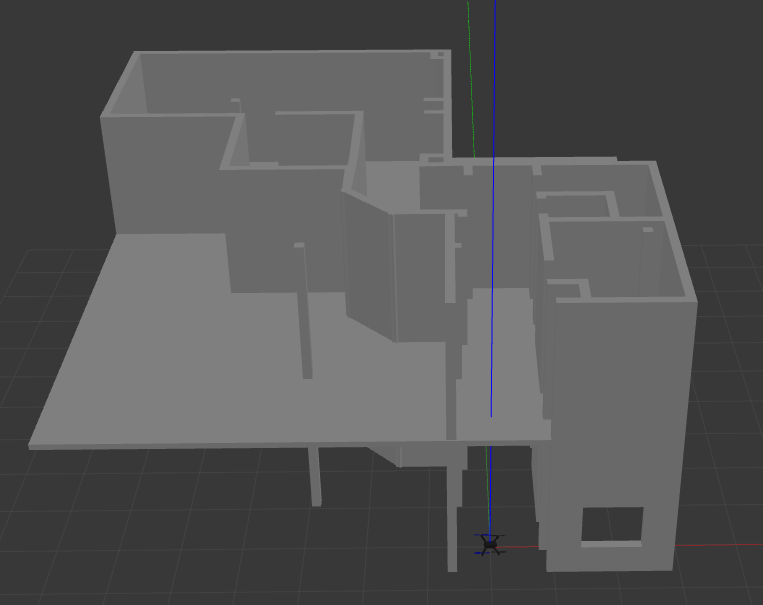
\includegraphics[height=62mm, keepaspectratio]{figures/building_2.png}}}$
    \caption{Two story building in Gazebo}
    \label{fig:building_floor_map}
\end{figure}

The second floor of the designed building is seen on figure \ref{fig:building_floor_map}. The ground
level has exactly the same floor map, except it also has a staircase in the top left room, windows
and what is important, it has a ceiling. Ceiling is expected to play an important role in 3D slam,
adding an extra reference point for vertical positioning. Using this building it is possible in 
the future to test the efficiency of 3D SLAM by flying up the stairs and around the second floor.

\subsection{Remote controller}
After following the previous steps and starting the simulation, the quadcopter with the LIDAR sensor
is being spawned at the entrance of the building, but it needs to be controlled to fly around the 
house. I chose to use a virtual controller that has been developed by a student at the laboratory 
of my department. The controller uses MAVROS topics to send and receive commands to and from the drone. 
Using this program, the quadcopter can be flown by using the PC keyboard. 

\begin{figure}[!ht]
    \centering
    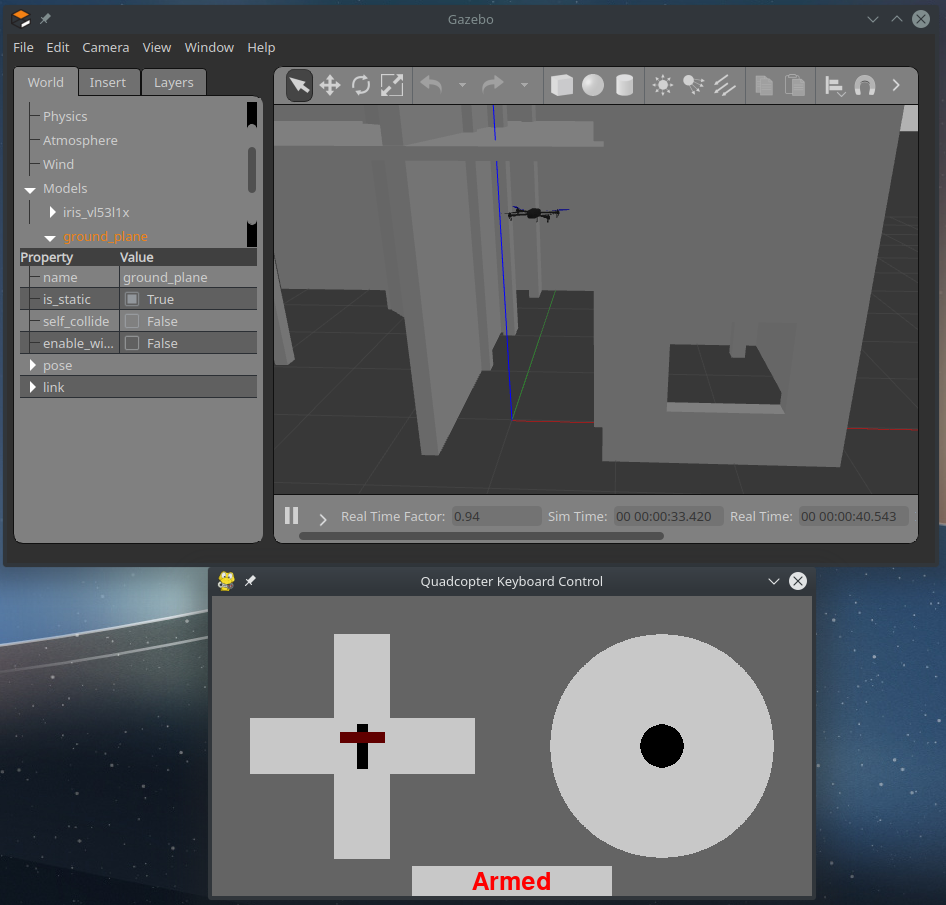
\includegraphics[width=100mm, keepaspectratio]{figures/fly_with_controller.png}
    \caption{Virtual remote controller for the simulated drone}
    \label{fig:remote_controller}
\end{figure}

For evaluation of SLAM the recorded flight time is kept low, so the data filtering and Cartographer 
can run faster. About 2 minutes of data is enough for comparing the performance of SLAM configurations
and further flights can take place to further test the evaluated configurations.

\section{Rosbag filtering}
Filtering is the process of reading rosbag messages, filtering LIDAR ranges to show behavior of the 
selected VL53L1X settings and writing the filtered data to a new bag file. Due to the high data rate, 
rosbags tend to take up lots of disk space. To preserve disk space and increase processing speed,
only necessary topics described in \ref{sect:cartographer_environment} are being written to the filtered file.

The recorded rosbag contains LIDAR measurements on two topics, the top sensor covers the top hemisphere,
the bottom one covers the bottom hemisphere. To simulate a VL53L1X sensor behavior, a field of view with a 
selected opening angle is cut out of the point cloud. Then an average of ranges inside this view is calculated.
The averaged distances are then maximized to a set maximum distance threshold and the sampling time is 
reduced according to the selected device settings. For simulating higher resolutions, the same methodology 
can be used, by using multiple field of views with smaller opening angles.

The raw measurements read from the collected rosbag are PointCloud type, but Cartographer requires 
PointCloud2 messages. At the end, the filtered points are converted to PointCloud2 and written
to the filtered bag file. 

\subsection{Update rate}
LIDAR messages are recorded in a rosbag at a certain rate and it needs to be down-sampled to match
the desired update rate. Every PointCloud message has a header field that contains the current time
at publish. During filtering each message is read from an input bag in order as they were published.
A PointCloud message is only considered for filtering, if the time difference between the last written 
and the current message is greater than the defined update rate. Otherwise the message is discarded.

Using this procedure the update rate will not match exactly the desired rate, but keeps data integrity
and order with other messages. 



\subsection{Field of View}
Each PointCloud message contains a complete scan from either the top or bottom sensor, that scan the 
top or bottom hemisphere accordingly. As the message type suggests, these ranges are represented by 
point clouds, a list of 3 dimensional point coordinates in reference to the sensor coordinate system. During 
angle filtering this point cloud is being down-sampled to lower resolution that simulates the sensors
placed on the quadcopter.

VL53L1X sensor has a cone shaped field of view in which the reflected signal is detected and converted to
a range measurement. To match this behavior, a cone shaped subset of the points are selected for further
processing. A point is selected if the angle between the point and the center of the field of view is less
than a predefined $\theta$ angle threshold.

\begin{figure}[!ht]
    \centering
    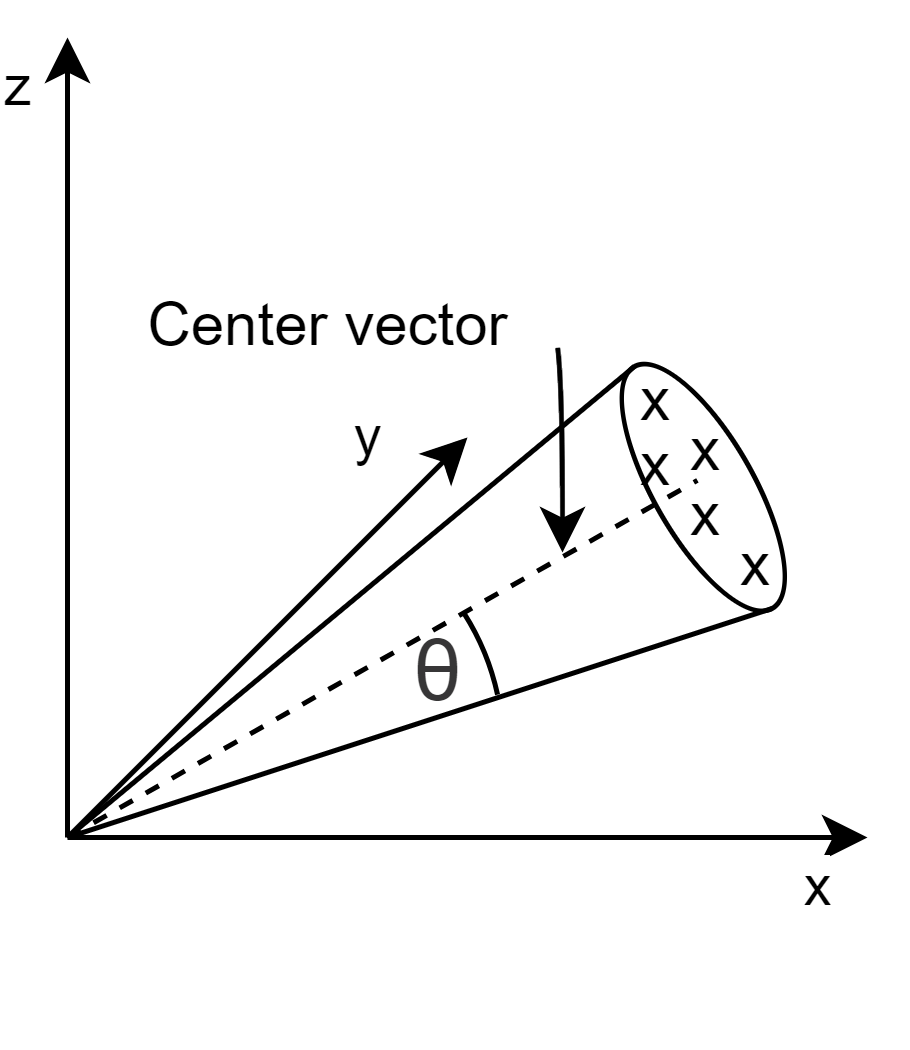
\includegraphics[width=80mm, keepaspectratio]{figures/data_angle_filter.png}
    \caption{Point cloud angle filter}
    \label{fig:data_angle_filter}
\end{figure}


The angle between two vectors, or in this case between a point from the point cloud and the center vector 
can be calculated using the dot product of the two. Equation \ref{eq:vec_product_angle} and 
\ref{eq:vec_product_coordinates} are two forms of dot product. These are used to derive equation 
\ref{eq:vec_product_final} that is used to calculate the angle. In this case vectors $\vec{u}$ and 
$\vec{v}$ are the center vector and a selected point from the point cloud. 


\begin{equation} \label{eq:vec_product_angle}
    \vec{u}\cdot\vec{v}=\left\|\vec{u}\right\|\left\|\vec{v}\right\|cos(\alpha)
\end{equation}
\begin{equation} \label{eq:vec_product_coordinates}
    \vec{u}\cdot\vec{v}=u_{x}v_{x}+u_{y}v_{y}+u_{z}v_{z}
\end{equation}
\begin{equation} \label{eq:vec_product_final}
    \alpha = cos^{-1}\frac{u_{x}v_{x}+u_{y}v_{y}+u_{z}v_{z}}{\left\|\vec{u}\right\|\left\|\vec{v}\right\|}
\end{equation}
\begin{equation} \label{eq:vec_length}
\left\|\vec{u}\right\| = \sqrt{u_{x}^{^{2}}+u_{y}^{^{2}}+u_{z}^{^{2}}}, \left\|\vec{v}\right\| = \sqrt{v_{x}^{^{2}}+v_{y}^{^{2}}+v_{z}^{^{2}}}
\end{equation}

For every point inside the point cloud this angle is calculated and points that have an angle less than the 
predefined $\theta$ are added to the list of points inside the field of view. As a final step average of the 
selected points is calculated. Points once again are represented by coordinates, therefore average is calculated 
by averaging the x, y and z coordinates resulting in the coordinates of a single point.

The steps described above are for the filtering a single sensor, but the same steps apply for multiple 
sensors. Higher resolutions are constructed by multiple field of views, with a lower angle threshold of 
$\theta$. Figure \ref{fig:data_angle_filter_high_res} shows an example for field of view selection for 
a resolution of 2x2. Field of view center line and angle threshold are not drawn, to keep the figure simple. 

\begin{figure}[!ht]
    \centering
    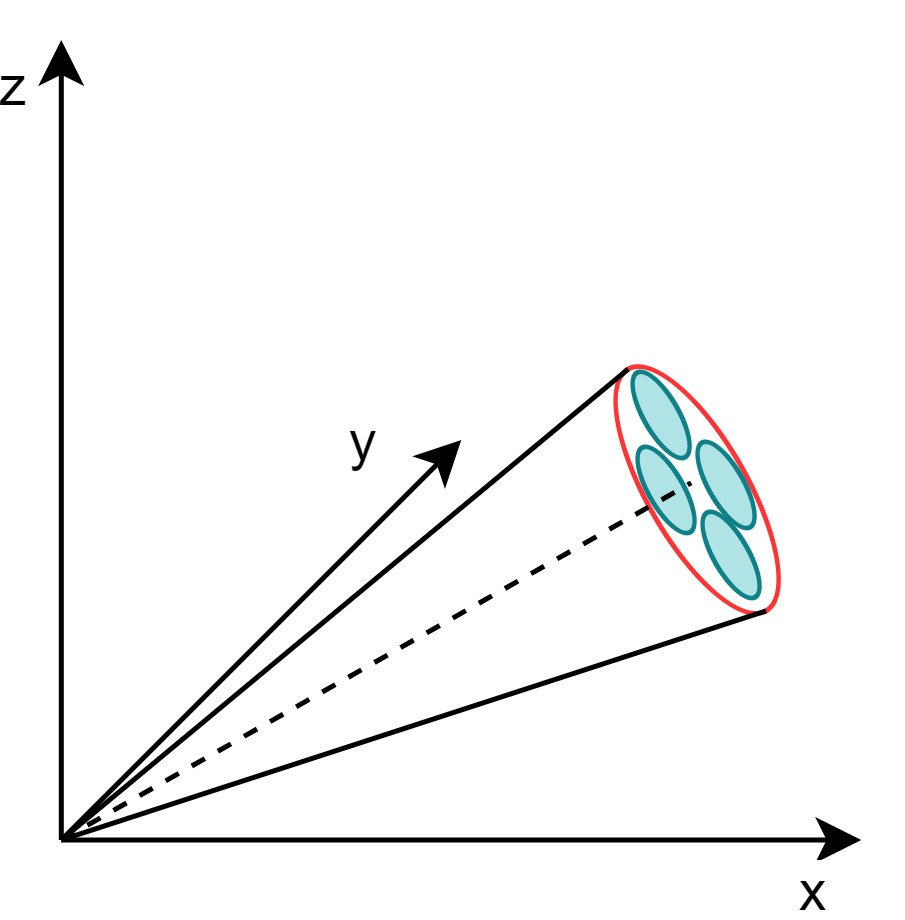
\includegraphics[width=60mm, keepaspectratio]{figures/data_angle_filter_high_res.png}
    \caption{Representation of 2x2 LIDAR resolution filtering}
    \label{fig:data_angle_filter_high_res}
\end{figure}

Points inside a PointCloud message always take the same order, therefore it's enough to filter 
for angles only once and use the indexes of these points from that on. This way lots of processing capacity
can be saved and it proved to be much more efficient on high number of simulated sensors.


\subsection{Distance filter}
Angle filter returns a single point for each predefined field of view. For each sensor it can mean a single 
point or up to 16 points in case of a resolution of 4x4. As the second step, distance filter receives these 
points and calculates the distance of each point from the origin, basically the same as calculation of length
of a vector. If the distance is greater than the defined maximum distance, the length of the vector
is shortened to the maximum distance. On figure \ref{fig:data_distance_filter} $p_{o}$ represents the 
point and $p_{s}$ is the shortened vector.

\begin{figure}[!ht]
    \centering
    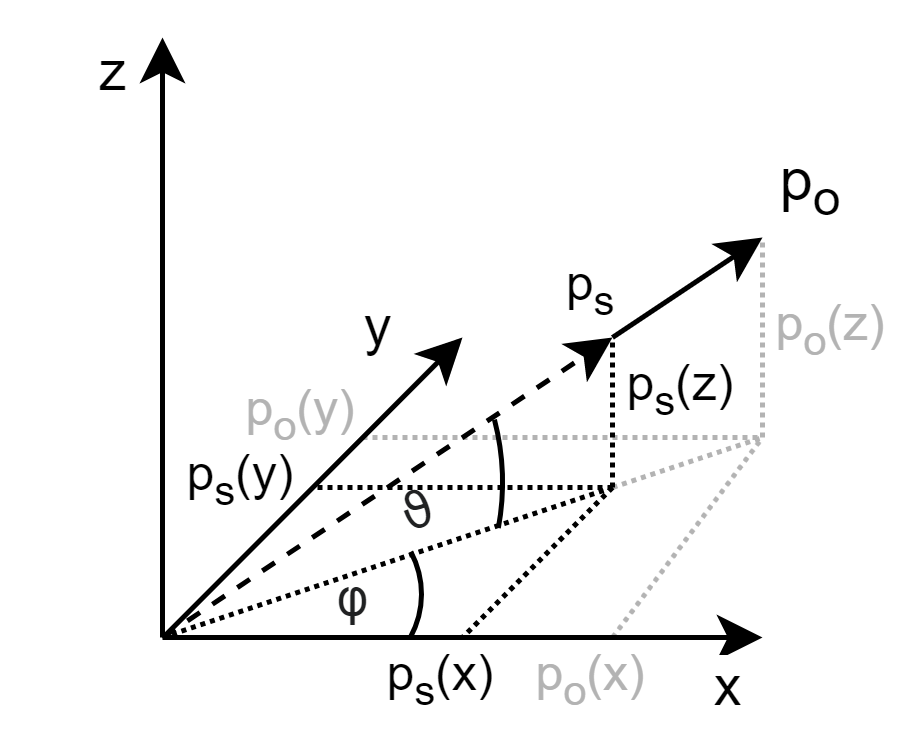
\includegraphics[width=70mm, keepaspectratio]{figures/data_distance_filter.png}
    \caption{Point cloud distance filter}
    \label{fig:data_distance_filter}
\end{figure}

\begin{equation} \label{eq:point_length}
    \left\|\vec{p_{o}}\right\| = \sqrt{{p_{o}^{x}}^{2}+{p_{o}^{y}}^{2}+{p_{o}^{z}}^{2}}
\end{equation}

To shorten the length of a vector, all three coordinates need to be recalculated in such way, that the attitude of
the vector does not change. To do so, vertical $\vartheta$ and horizontal $\varphi$ angles for vector $p_{o}$
are calculated using equation \ref{eq:vec_elevation} and \ref{eq:vec_horizontal}.

\begin{equation} \label{eq:vec_elevation}
    \vartheta=tan\frac{p_{o}^{z}}{\sqrt{{p_{o}^{x}}^{2} + {p_{o}^{y}}^{2}}}
\end{equation}
\begin{equation} \label{eq:vec_horizontal}
    \varphi=tan\frac{p_{o}^{y}}{p_{o}^{x}}
\end{equation}

Using the vertical and horizontal angles, the coordinates of the shortened $p_{s}$ is calculated using 
trigonometric equations \ref{eq:vec_new_coordinate_x}, \ref{eq:vec_new_coordinate_y} 
and \ref{eq:vec_new_coordinate_z}.

\begin{equation} \label{eq:vec_new_coordinate_x}
    p_{s}^{x} = d_{max} \cdot cos\vartheta \cdot cos\varphi
\end{equation}
\begin{equation} \label{eq:vec_new_coordinate_y}
    p_{s}^{y} = d_{max} \cdot cos\vartheta \cdot sin\varphi
\end{equation}
\begin{equation} \label{eq:vec_new_coordinate_z}
    p_{s}^{z} = d_{max} \cdot  sin\vartheta
\end{equation}



\section{Cartographer environment} \label{sect:cartographer_environment}
Cartographer can be installed on Ubuntu operating system easily by using the apt-get tool, but this
method would overwrite the system installed Protobuf with a newer version. Protobuf is used by 
Gazebo and it requires a certain version, replacing it with another version causes incompatibility 
and simulations cannot be started. For this reason I have installed Cartographer and Cartographer\_ros
packages inside a Catkin workspace and set them to use locally installed Protobuf inside the same
workspace. Using these settings, Cartographer and Gazebo can be used on the same PC.

\begin{figure}[!ht]
    \centering
    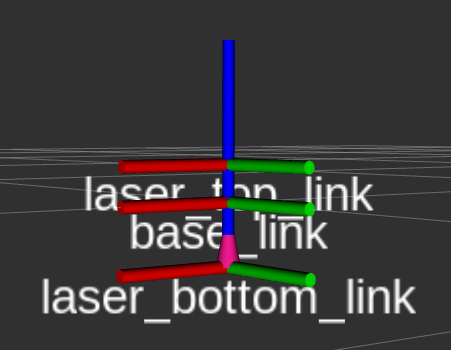
\includegraphics[width=70mm, keepaspectratio]{figures/cartographer_tf_setup.png}
    \caption{Cartographer top, bottom LIDAR and IMU link relations}
    \label{fig:cartographer_tf_setup}
\end{figure}


To attach the LIDAR sensors onto the simulated quadcopter in Gazebo, two links have been introduced that
connect to the base\_link of the drone, one on the top and one on the bottom. The LIDAR scanner messages 
are sent in reference to these links and therefore Cartographer needs to know the transformation from the
sensor frames to the base\_link frame. Two official packages are required called robot\_state\_publisher
and joint\_state\_publisher. These take a robot\_description parameter that can be set using an urdf file 
and they start publishing the link and joint relations. Besides the LIDAR holder links, a link for IMU 
transformation is also need to be added. The simulated IMU in the PX4 repository is used and it is located in 
the origin of base\_link. Laser\_top\_link is located 6cm up, laser\_bottom\_link is located 10cm down
on the z axis in reference to base\_link as seen on \ref{fig:cartographer_tf_setup}.

\begin{figure}[!ht]
    \centering
    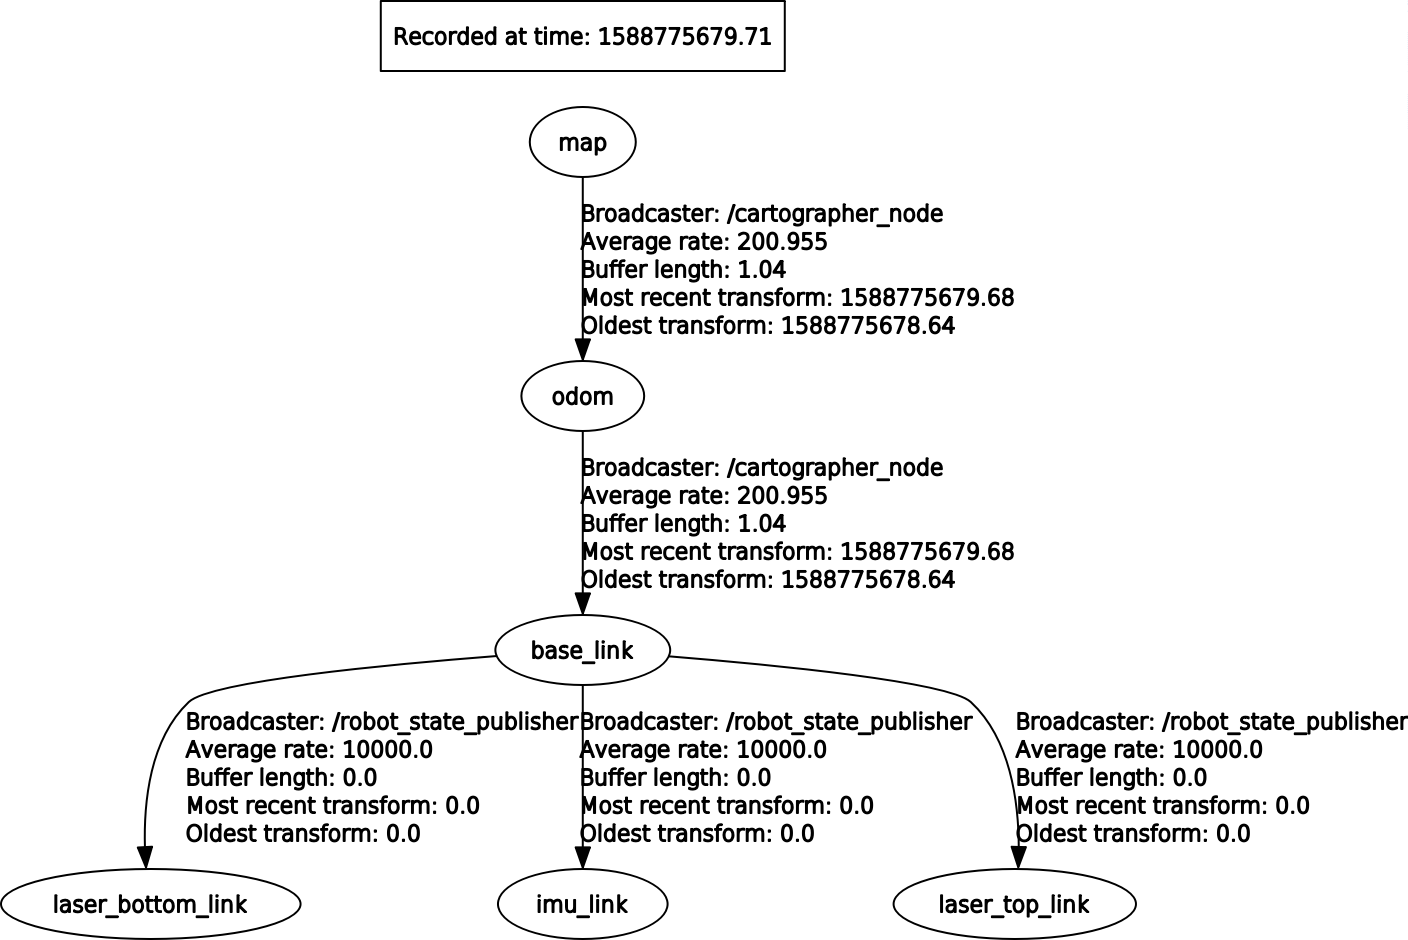
\includegraphics[width=110mm, keepaspectratio]{figures/cartographer_tf_tree.png}
    \caption{Cartographer tf tree}
    \label{fig:cartographer_tf_tree}
\end{figure}


While running Cartographer on filtered data, the following tf tree is built as on \ref{fig:cartographer_tf_tree}.
Transformations between map, odom and base\_link are published by Cartographer and the rest is published 
from the created urdf file. This tf tree matches the recommendation from the Cartographer documentation
website \cite{CartographerDocumentation}.

IMU input for 3D mapping is a must and optional for 2D mapping. Cartographer waits for IMU to be supplied 
on topic /imu. PX4 simulation publishes IMU data to /mavros/imu/data, but this topic can be remapped to /imu
using the launch file without the need of any extra nodes. Filtered range messages with PointCloud2 type 
can be accessed on topics /points2\_1 and /points2\_2. List of nodes and interactions via topics can be 
seen on figure.

\begin{figure}[!ht]
    \centering
    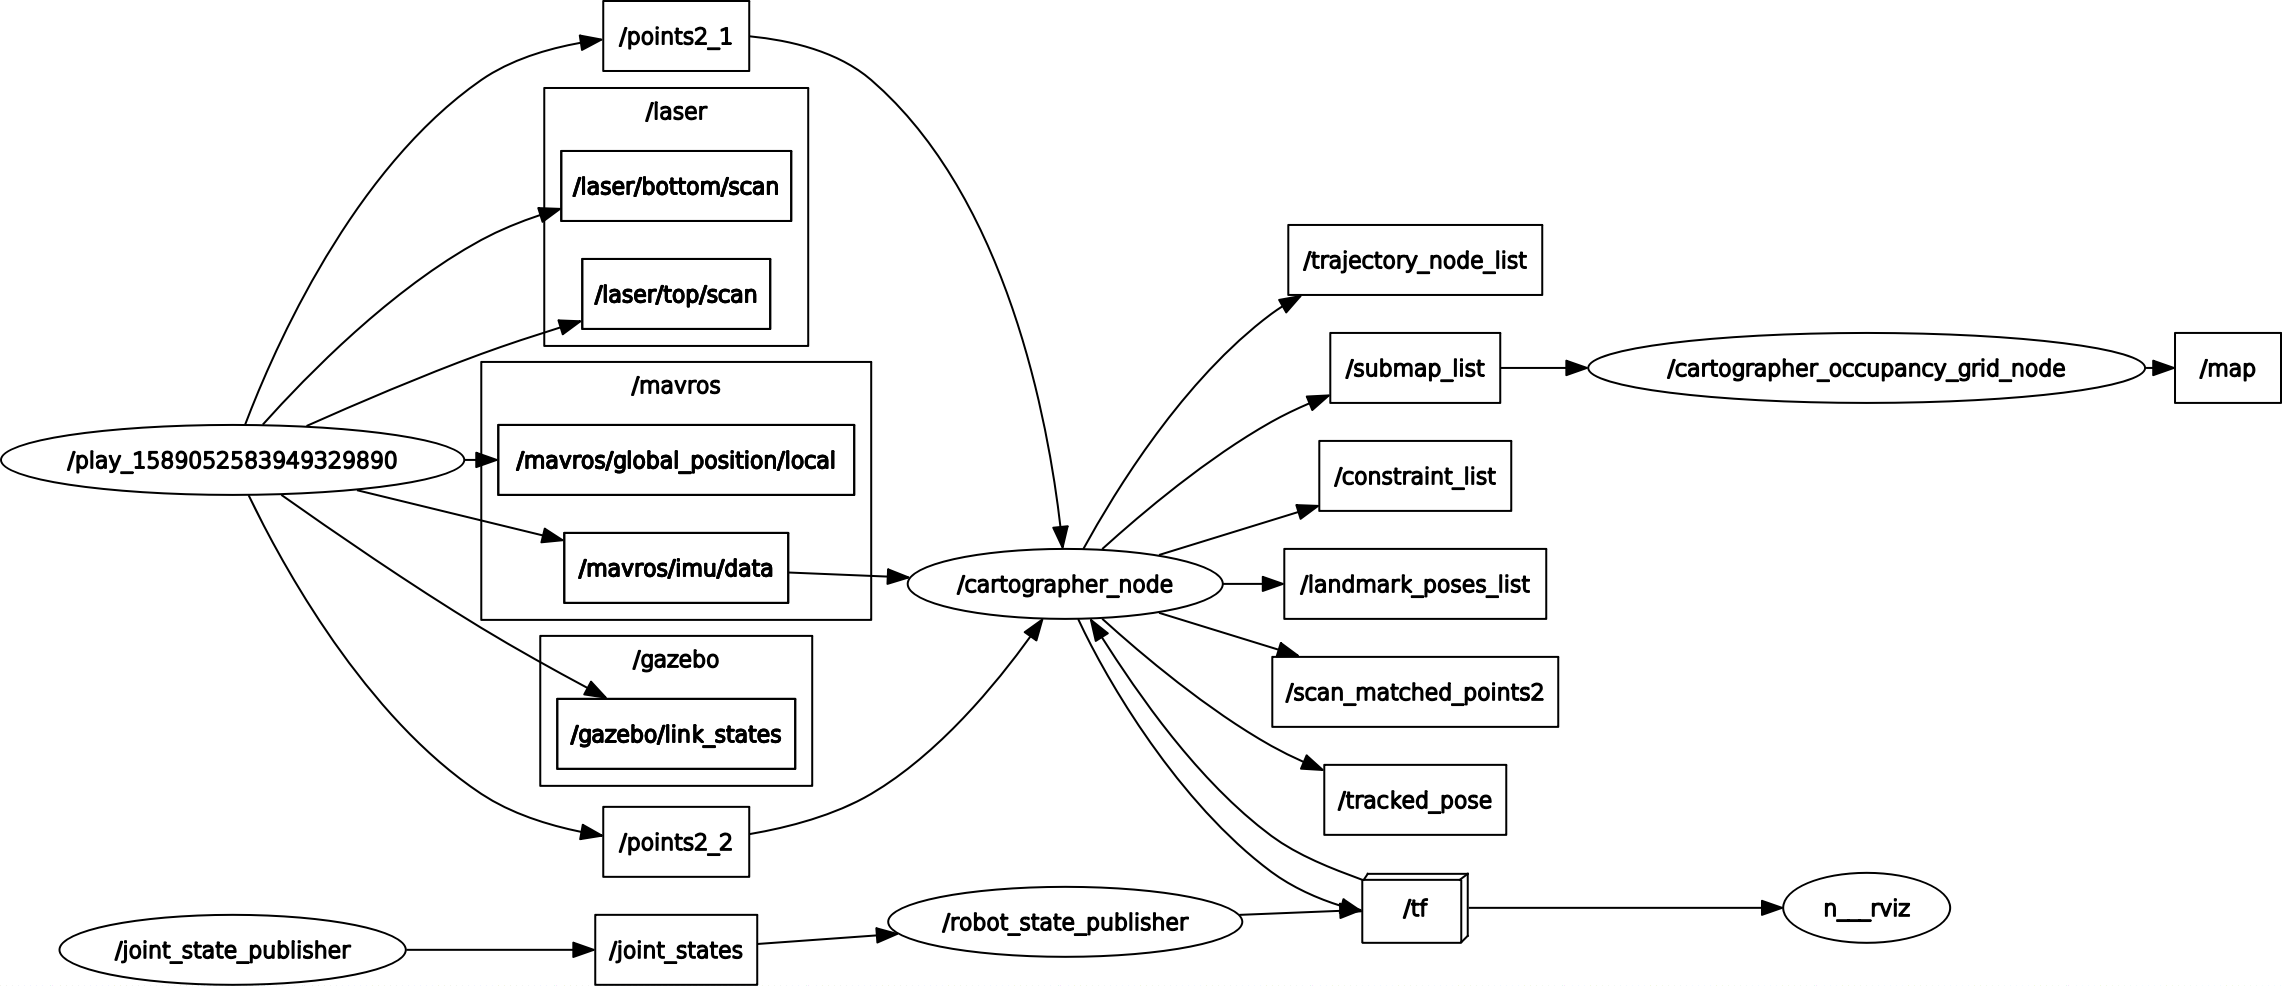
\includegraphics[width=140mm, keepaspectratio]{figures/cartographer_nodes.png}
    \caption{Cartographer nodes and topics}
    \label{fig:cartographer_nodes}
\end{figure}

\subsection{Configuration and tuning}
Cartographer can be configured using a lua configuration file. Multiple range measurement types are 
supported, but the filtered rosbag contains PointCloud2 messages on two topics. The num\_point\_clouds 
parameter is set to 2 to match the two topics coming from the top and bottom sensors. 

Cartographer applies a bandpass filter on the incoming range messages to filter out irrelevant 
measurements. In every case max\_range parameter needs to be set a bit lower, than the maximum distance
parameter used for filtering. This is important, because the algorithm inserts a range with a distance 
under max\_range as a hit, but inserts anything above as a miss. Wrongly setting this parameter results
in adding all range measurements as hits and no misses will be inserted that will confuse cartographer.

Each sensor setup require the SLAM algorithm to be tuned and therefore a new configuration file is 
created for every setup being tested. Tuning starts with setting POSE\_GRAPH.optimize\_every\_n\_nodes to
0 to disable global SLAM. Good and clear submaps are needed for global SLAM to find loop closures.
Submaps are the building blocks of maps. On small maps like the building I chose for LIDAR setup 
evaluation, global SLAM is not making much difference, but when tuning submaps it can cause unwanted
artifacts that are hard to differentiate from submap errors.

\begin{figure}[!ht]
    \centering
    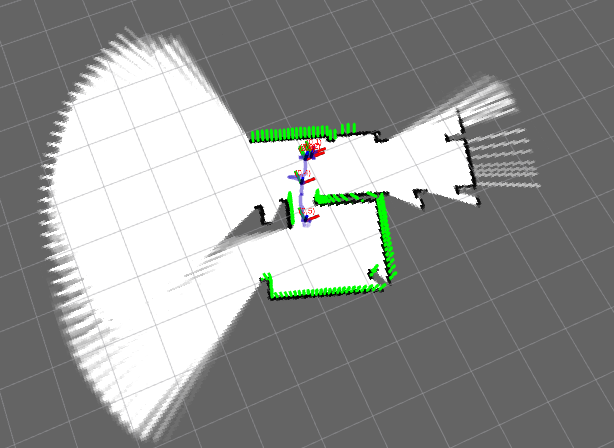
\includegraphics[width=80mm, keepaspectratio]{figures/cartographer_submaps.png}
    \caption{Building of submaps visualized in rviz}
    \label{fig:cartographer_submap_building}
\end{figure}

Typically a small number of parameters need to be tuned for submaps to be working. These are the following:
\begin{itemize}
    \item TRAJECTORY\_BUILDER\_nD.ceres\_scan\_matcher.translation\_weight
    \item TRAJECTORY\_BUILDER\_nD.ceres\_scan\_matcher.rotation\_weight
    \item TRAJECTORY\_BUILDER\_nD.ceres\_scan\_matcher.occupied\_space\_weight 
    \item submaps.num\_range\_data
\end{itemize}
The first parameter sets how high the cost is for cartographer to move the a scan. In my experience,
it needs to be set low when used on a drone, because it changes place quickly. The second parameter sets 
how much trust should be put on the IMU data. The lower this parameter is set, the easier it is to 
rotate a scan and be matched against other scans in the submap. Occupied space weight is sets the 
trust in the LIDAR sensor. I haven't found this parameter particularly useful. Changing the submap 
size, by num\_range data parameter is important, because by changing the update rate, different 
number of range measurements are needed, while the submap scope should not change.


\subsection{Trajectory extraction}\label{sect:trajectory_extraction}
Evaluating the mapping quality is complex relative to evaluating the location tracking performance
of a SLAM setup. Gazebo provides a topic where all link states are published and this transformation
can be used as ground truth and trajectory extracted from SLAM can be compared to it.

I found two ways to extract trajectory from Cartographer. One is to create a node that subscribes to
/tf topic and saves map to base\_link transformations that is published by Cartographer. The other
way is to save the internal variables of the algorithm into a pbstream file and use a script to read
the pose estimations from there. For some reason published transformations proved unreliable on my
tests, but the published trajectory node list on topic /trajectory\_node\_list contains the correct
pose estimates.

Cartographer can run in mapping mode and pure localization mode. In localization mode, it
only stores variables for several seconds and for this reason the pbstream file does not contain
the whole trajectory. In this mode, trajectory can only be extracted by saving pose from 
/trajectory\_node\_list topic. For mapping mode I have decided to use trajectory extracted from 
the pbstream file.




\section{SLAM performance evaluation}
As the name SLAM suggests and described before, it focuses not only on mapping but simultaneous 
localization too. On the other hand evaluation of mapping and localization can be done separately.
This thesis mainly focuses on localization, while mapping is secondary. For this
reason only localization accuracy is being measured quantitatively and mapping accuracy is 
only evaluated by visual inspection.

By SLAM performance I mean the accuracy of the localization of each setup. While the number of 
sensors used and their placement are important parameters of a setup, these are not included in
the evaluation process. The goal of evaluation is to give an objective measure of the localization
accuracy, independently from the hardware implementation. 

In order to compare SLAM setups, an objective measure of goodness need to be introduced. Based 
on this quantitative measure or score, the setups can be compared. Localization is chosen to be 
the main focus and it can be measured by comparing the trajectory output of the algorithm
to a ground truth. 
As described in \ref{sect:trajectory_extraction} the list of estimated poses can be extracted 
from the pbstream file, provided by Cartographer. On topic /gazebo/link\_states transformations
are available for base\_link that were used for visualization of the quadcopter in Gazebo. 
This data is the most accurate position information available and therefore it is chosen to be used as
ground truth for the drone's trajectory.

Cartographer can either be run in normal operation or in pure localization mode. Pure localization
mode means, that the algorithm only keeps a small number of submaps in the memory at a time and 
matches them against submaps of a previously built map. Further building of the map is disabled 
in this mode and submaps will be discarded once they become obsolete. 

In case of Cartographer, pure localization mode is basically a stripped down version of the normal
operation mode and for this reason building good quality submaps is also essential for the algorithm to 
be working accurately. Tuning procedure can happen in normal operation mode and then used in 
localization mode afterwards. A setup that is able to produce good quality submaps, means it
will also work accurately in localization mode, therefore I chose to evaluate and compare setups
in normal operation mode. 

\subsection{Down-sampling}
Link states are much more often published by gazebo, than the extracted trajectory by Cartographer. 
To compare the two sets of data, they need to have the same size. To achieve that, ground truth
data is down-sampled to the size of the SLAM trajectory.

\subsection{Offset compensation}
Before error calculations, the SLAM trajectory needs to be rotated and moved to align with the
ground truth data. The distance and rotation offsets are calculated using the first pose from both
datasets. The distance offset equals to the difference of the x,y and z coordinates of the poses,
while the rotation offset is the difference between the yaw angles. In my initial tests there were 
no roll and pitch offsets present, because of the use of IMU of Cartographer. 

To compensate for different starting points, the calculated offsets on each axis needs to be 
subtracted from every data point present in SLAM trajectory. For the rotation offset, the 
following trigonometric formulas are used, where $\theta$ is the offset on yaw angle.

\begin{equation}\label{eq:rotation_x}
    x'=x\cdot cos\theta + y\cdot sin\theta    
\end{equation}

\begin{equation}\label{eq:rotation_y}
    y'=-x\cdot sin\theta + y \cdot cos\theta
\end{equation}

\begin{figure}[!ht]
    \centering
	$\vcenter{\hbox{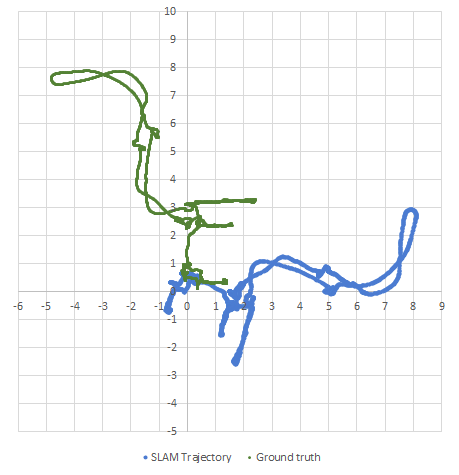
\includegraphics[width=70mm, keepaspectratio]{figures/trajectory_example_uncompensated.png}}}$
    $\vcenter{\hbox{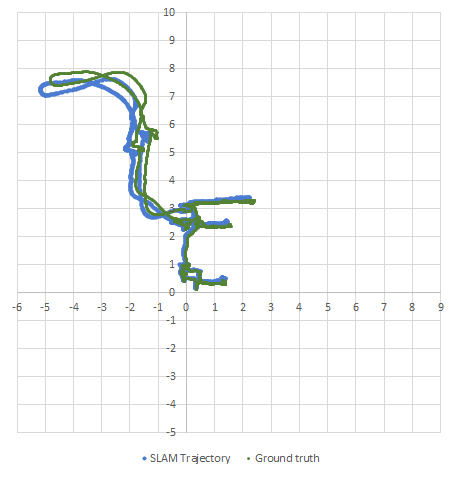
\includegraphics[width=70mm, keepaspectratio]{figures/trajectory_example_compensated.png}}}$
    \caption{Extracted trajectory against ground truth before and after offset compensation}
    \label{fig:before_after_offset}
\end{figure}





\subsection{Trajectory error calculation}
As a quantitative measure I chose to use the error of the estimated trajectory, calculated using 
the RMS error formula \ref{eq:rms_formula}. The RMS error is calculated on all three axes, 
$\hat{c_i}$ is one coordinate of the estimated pose the and $c_i$ is the according coordinate 
of the pose from ground truth trajectory.

\begin{equation}\label{eq:rms_formula}
    RMSError(c)=\sqrt{\frac{\sum_{i=1}^{n}(\hat{c_i}-c_i)^2}{n}}
\end{equation}

After calculating RMS error on all three axes, to get the cumulated trajectory error the 
values are summed. The result is a single positive number in meters, that can be used to
compare the accuracy of different SLAM setups.


\section{Complete workflow}

\begin{figure}[!ht]
    \centering
    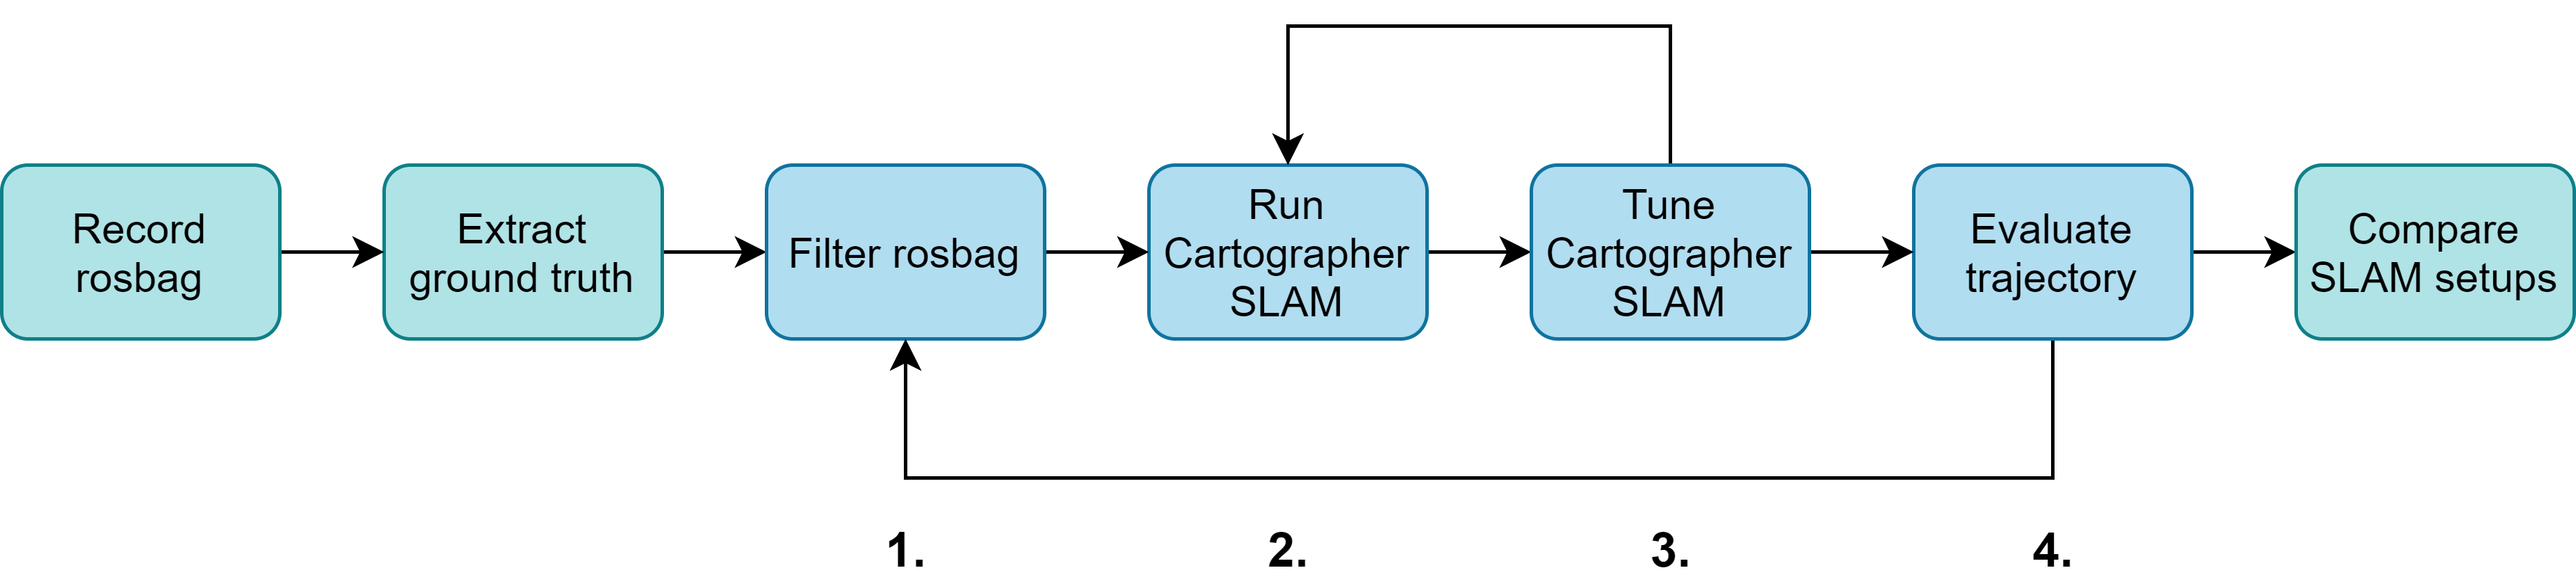
\includegraphics[width=140mm, keepaspectratio]{figures/workflow.png}
    \caption{Complete workflow}
    \label{fig:workflow}
\end{figure}

The complete workflow is as seen on figure \ref{fig:workflow}. As preliminary steps a rosbag is
recorded and ground truth trajectory is extracted from it. After this step, all SLAM setups
will be evaluated based on this data. To evaluate a selected setup, first the rosbag is
filtered according the layout and sensor settings. Then Cartographer SLAM is run and 
tuned for this dataset. At step 4 the RMS error is calculated based on the estimated 
trajectory from the SLAM algorithm. 

These 4 steps are done for every selected SLAM setups and as a final step the results 
will be compared.


  
 
% Roslaunch is a tool for easily launching multiple ROS nodes, as well as setting parameters. Nodes can
% be started one by one, but it is more efficient to use a launch file to describe nodes and parameters 
% to start.

% To make starting of simulations easy and consistent, I have created a new launch file and placed


% that collects the models and worlds I have created.


\newpage


\section{Plans for hardware implementation}
On a real-life drone, the communication of LIDAR sensors and measurement forwarding to ROS topics need
to be solved. There needs to be a device that communicates with the VL53L1X LIDAR sensors using I2C
protocol and forwards messages to a ground station that handles data collection and processing.

The data collector device needs to be fast enough to keep up with the pace of 10-20 sensors,
each with a maximum of 50Hz update rate. The distance data from VL53L1X sensor consists of 12bytes, 
so by designing for 20 sensors with 50Hz update rate generate about 12kb per second data rate. This 
load is calculated using the effective data size, but on the I2C bus other configuration messages 
need to be sent, which means even higher load.

To evaluate the SLAM algorithms on real-world measurements, data needs to be collected. 
For evaluation it is not necessary to send data in real-time on wireless network, but saving 
data on an SD card serves this purpose. Logging on SD card has low complexity and high speed. 

PX4 is an open-source firmware, it seems an easy choice to use the Pixhawk 4 autopilot board 
as a data collector device. It has an SD card slot for logging and I2C connectors available to
communicate with the LIDAR sensors and even comes with an I2C splitter board to connect more sensors.
The microcontroller inside Pixhawk 4 is powerful, it has an ARM Cortex-M7 core running on 216MHz. 
It is used to run highly timing sensitive control loops to produce actuator values for stable flights,
besides many other tasks. If these control loops are delayed by other processes, that can 
cause instable flight or even crash.

Because of lack of deep understanding of PX4 firmware, to make sure that timing of control loops 
are untouched, I decided to design a standalone data collector, using a dedicated microcontroller that
handles I2C communication with the LIDAR sensors and writes data to an SD card using SPI protocol.

\subsection{Standalone data collector design}
In I2C protocol every device needs to have a 7 bit address, that needs to be unique on every
I2C line. VL53L1X sensor has a default address of 0x29 when the sensor is booted, but it can be changed
by using I2C commands. Address conflicts need to be avoided by having exactly 1 sensor active per channel.
It is hard to find a microcontroller that has 20 I2C buses, one for each sensor, so multiple sensors
need to be placed on the same bus. By having multiple sensors on the same channel, the sensors need to 
be released from reset one by one to change their addresses, this way address conflicts can be avoided.
VL53L1X can be kept in reset by pulling its shutdown pin to ground and activated by bringing it to 
supply voltage. 

The sensors have altogether 4 lines that need to be driven: 2 I2C, 1 shutdown and 1 interrupt pin.
In the simplest case, by connecting each wire to the microcontroller, 80 wires would be needed for 
20 devices and would take 42 pins of the microcontroller. Although it is possible to find a microcontroller 
that has enough pins and connect all sensors one by one to the same I2C bus, but by grouping them 
into groups of 5 and connecting each group to different I2C buses, a significant improvement can be 
achieved on the number of connections. 

Sensors on different I2C buses can have the same address, therefore the same 5 addresses can be used
in each group. Shutdown pin of sensors sharing the same addresses can be common, this way number of
wires needed for shutdown is reduced from 20 to 5.

\begin{figure}[ht]
    \centering
    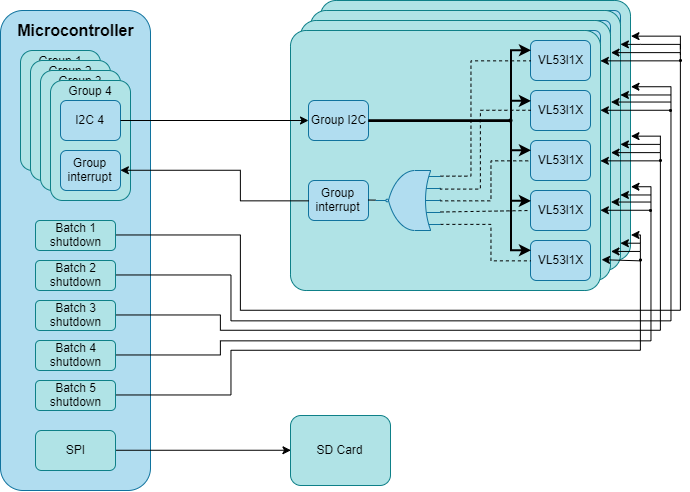
\includegraphics[width=100mm, keepaspectratio]{figures/data_collector.png}
    \caption{Design of data collector}
    \label{fig:data_collector}
\end{figure}

Handling 20 interrupt lines can be overwhelming for any CPU, while bringing little or no extra
benefit. Using only one interrupt line per group is enough to signal the microcontroller that 
measurements are ready to be read out in all sensors in that group. Interrupt pins are active-low,
so to produce the group interrupt signal a NOR gate needs to be used. When the state of all interrupt
pins are low, group interrupt signal will become logical 1 and 0 otherwise.

In the simplified design seen on figure \ref{fig:data_collector} only 17 wires are connected to
the microcontroller, while no functionality is lost. This solution also makes software development
easier and the built system is clearer.



